\section{État de l'art}
\label{sec:etat_art}
    Il n’existe pas de plateforme dédiée qui référence et permette d’accéder exclusivement à des documents de presse ancienne de toutes
    provenances (une est consacrée aux journaux anciens du Royaume-Uni spécifiquement). Cependant
    on peut constater de plus en plus un gain d’intérêt (notamment suite à des événements comme les 100 ans de la Grande Guerre)
    à accéder à des documents anciens qui peuvent être des actes de naissance, des registres d’état civil, des registres matricules ...
    et plusieurs plateformes ont vu le jour ces dernières années, permettant de consulter des documents de ce genre.


        \subsection{Archives des Yvelines}
        \label{subsec:yvelines}
        Archives Yvelines” est une plate-forme d’archivage et de consultation de documents antérieures à 1790
        concernant les communes des Yvelines, rassemblées pendant la Révolution. La plate-forme comporte près
        de 2 167 410 pages parmi lesquelles des archives publiques et privées, ouvrages de bibliothèques, titres de presse locale,
        photographies et cartes postales, maquettes, pages numérisées, documents communiqués en salle de lecture, expositions virtuelles...

        La plate-forme des archives des Yvelines permet de faire une recherche plus ou moins affinée en fonction d’une thématique
        (registres paroissiaux, recensement de population, répertoires de notaires, presse ancienne,. . . ) ou en fonction de la commune.

        \begin{figure}[H]
            \centering
            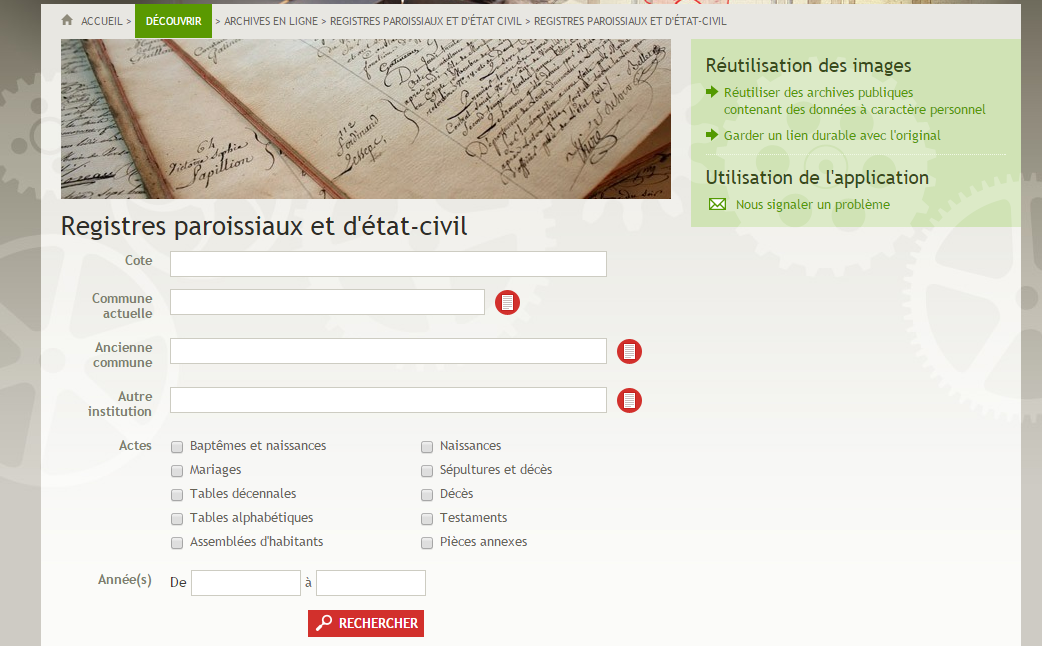
\includegraphics[width=1\textwidth]{figure/screen_yvelines_recherche.png}
            \caption{Capture d'écran de la recherche sur Archives Yvelines}
            \label{fig:yvelines_recherche}
        \end{figure}

        Par exemple, pour une recherche dans les registres paroissiaux et d’état civil (illustrée par la figure ci contre),
        il est possible de choisir plusieurs critères d’affinement de la recherche comme la cote, le type d’acte, la période...
        La recherche par commune donne accès à tous les différents documents d’une commune.

        Après avoir accédé au document, il est possible d’effectuer plusieurs actions en fonction du type de document.
        Par exemple pour les documents numérisés, les principales actions sur le document sont le zoom, le téléchargement,
        la récupération du lien, l’ajout dans un panier, le signalement d’une erreur, l’annotation et l’impression (confère la figure ci-dessous).

        Il existe certains documents comme les fiches concernant les navires de guerre où il n’est pas possible d’effectuer
        une action pendant la consultation.

        \begin{figure}[H]
            \centering
            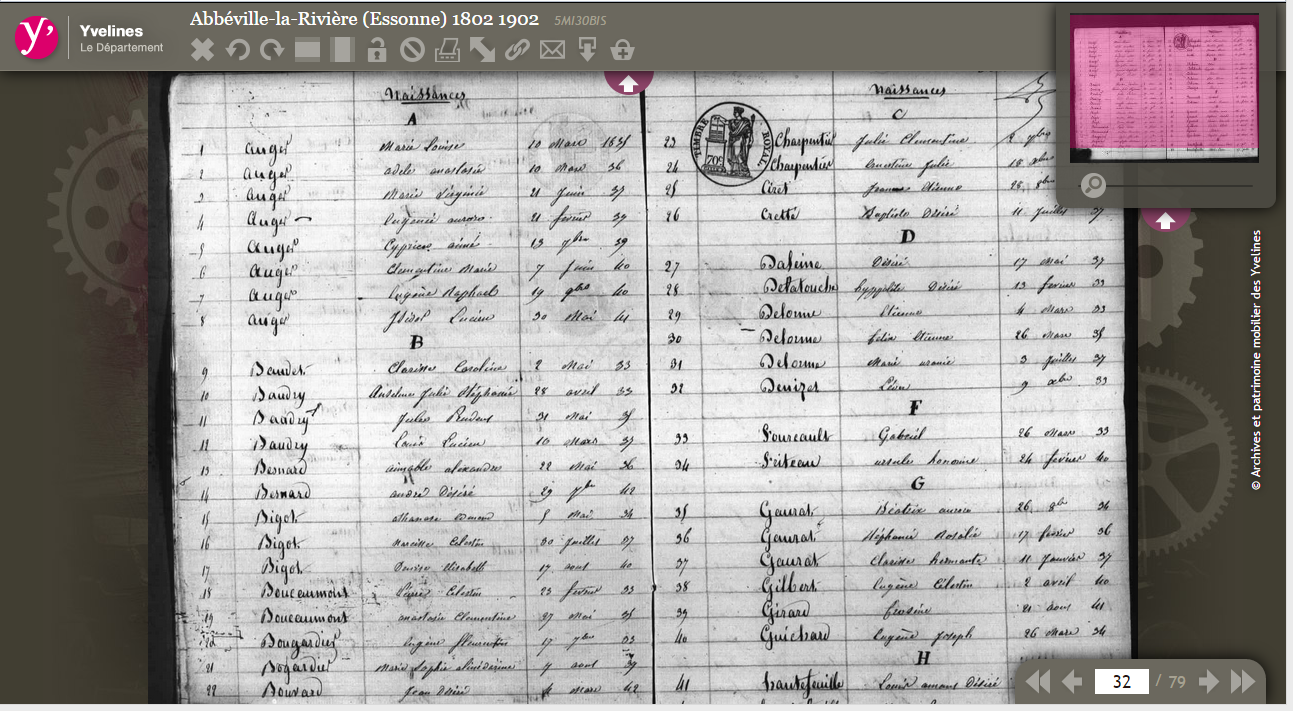
\includegraphics[width=1\textwidth]{figure/screen_yvelines_document.png}
            \caption{Capture d'écran de l'outil de visualisation d'un document sur Archives Yvelines}
            \label{fig:yvelines_doc}
        \end{figure}

        Concernant la consultation de presse ancienne (qui est l’objectif de notre projet), Archives Yvelines propose en plus
        de toutes les actions énumérées plus haut, une recherche en plein texte dans les journaux. La plate-forme propose
        aussi une annotation collaborative pour permettre des recherches par indexation dans la presse ancienne. Le service d’annotation
        n’est disponible que pour les utilisateurs possédant un compte ; ce qui peut être assez contraignant pour certains utilisateurs.

        \subsection{Mémoire des hommes}
        \label{subsec:memoire}
        Mémoire des hommes” est aussi une plate-forme de consultation d’anciens documents
        et qui a été inaugurée en 2003. Elle comporte essentiellement des fiches numérisées concernant
        les militaires français acteurs des conflits tels que la Première et Seconde Guerre mondiale,
        la guerre d’Indochine, la guerre de Corée, ou encore la guerre d’Algérie.

        Le site “Mémoire des hommes” permet d’effectuer une recherche soit grâce aux indexations
        réalisées à l’aide des annotations des utilisateurs, soit par thématique de guerre.
        Il est possible d’affiner la recherche avec des informations concernant la personne telles que le nom,
        la date de naissance, le lieu de naissance, le département, ...

        Les actions réalisables sur les documents sont identiques à celles de la plate-forme
        des archives des Yvelines, les deux plate-formes utilisant le même outil pour la visualisation
        de documents.

        Le site ‘Mémoire des hommes’ possède une petite particularité qui est la cartographie pour
        certaines guerres comme la guerre de Corée ; cartographie sur laquelle est localisée chacune
        des batailles de la guerre, la période et le nombre de décès.

        \begin{figure}[H]
            \centering
            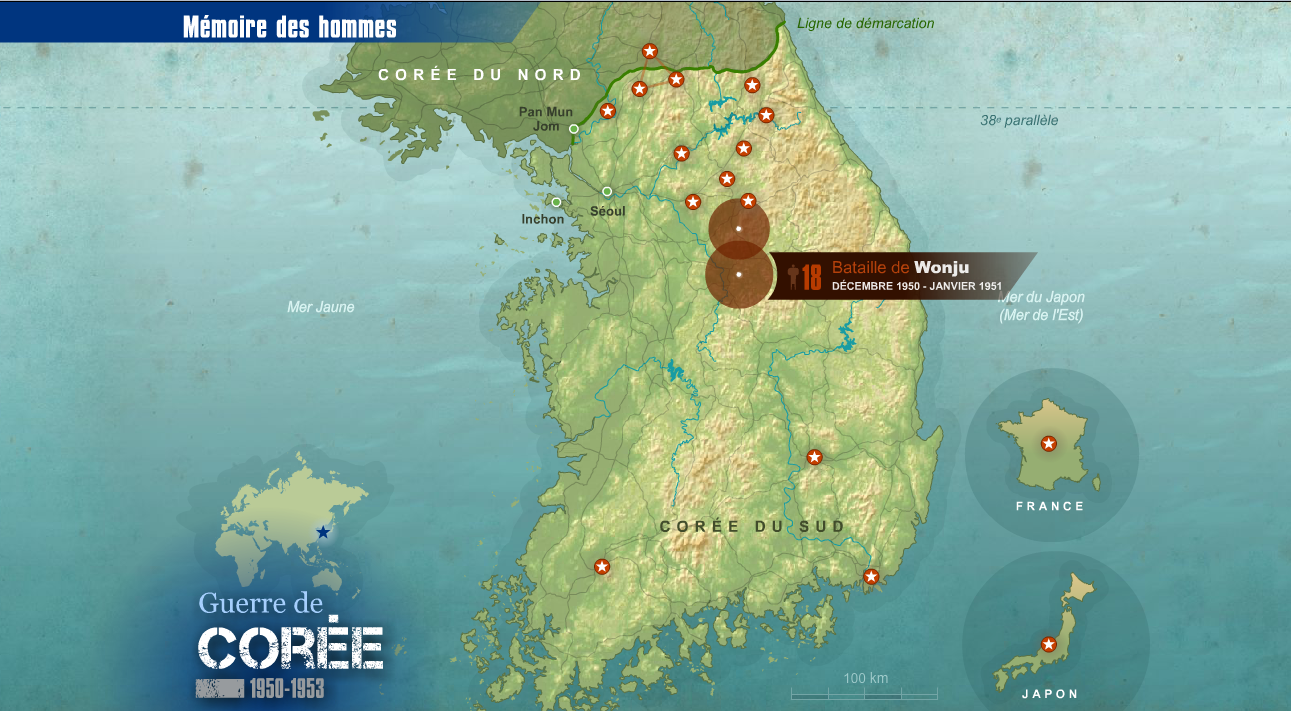
\includegraphics[width=1\textwidth]{figure/screen_memoire_hommes.png}
            \caption{Capture d'écran de la cartographie Mémoire des hommes}
            \label{fig:memoire_hommes}
        \end{figure}

        \subsection{Numdam}
        \label{subsec:numdam}
        C’est un programme de la Cellule de coordination documentaire nationale pour les mathématiques (Mathdoc) soutenant des revues
        de mathématiques en rendant leurs archives consultables sur internet. Les revues sont scannées en haut définition et mises
        à disposition en format djvu ou pdf. Le texte des pdfs est protégé contre la copie mais on peut cependant faire
        une recherche de mots dessus. On note la présence du format djvu adapté aux liseuses électroniques, ce dernier n’est
        pas protégé contre la copie du texte. La bibliothèque est relativement “pauvre” avec une collection de 36 journaux, 32 séminaires et 5 mémoires.

        \subsection{Gallica}
        \label{subsec:gallica}
        C’est la bibliothèque numérique de la Bibliothèque nationale de France, elle est en ligne depuis 1997.
        La bibliothèque est très riche de contenu avec aujourd’hui plusieurs millions de documents
        et chaque semaine des milliers de nouveautés. On peut consulter les œuvres directement sur le site,
        nous avons accès à tout un panel de commandes pour naviguer dans l’ouvrage: flèches suivant/précèdent,
        zoom, rotation, plein écran, recherche sur le texte, mode d’affichage, téléchargement, partage,
        signaler une anomalie. On a accès à des légendes en rapport avec l’œuvre et dans le même panel
        au texte où l’on peut effectuer une recherche plein texte. Cependant, le texte, reconnu avec un OCR
        (Optical character recognition - Reconnaissance optique de caractère), est parfois inexact.
        Gallica informe avoir eu recourt à deux types d’OCR, un OCR brut sans intervention humaine ou un OCR
        avec montée en qualité du texte ou celui-ci est amélioré par une correction manuel. On peut ainsi
        attendre un taux qualité cible de 96 à 99.9\% avec l’OCR le plus qualitatif.

        \begin{figure}[H]
            \centering
            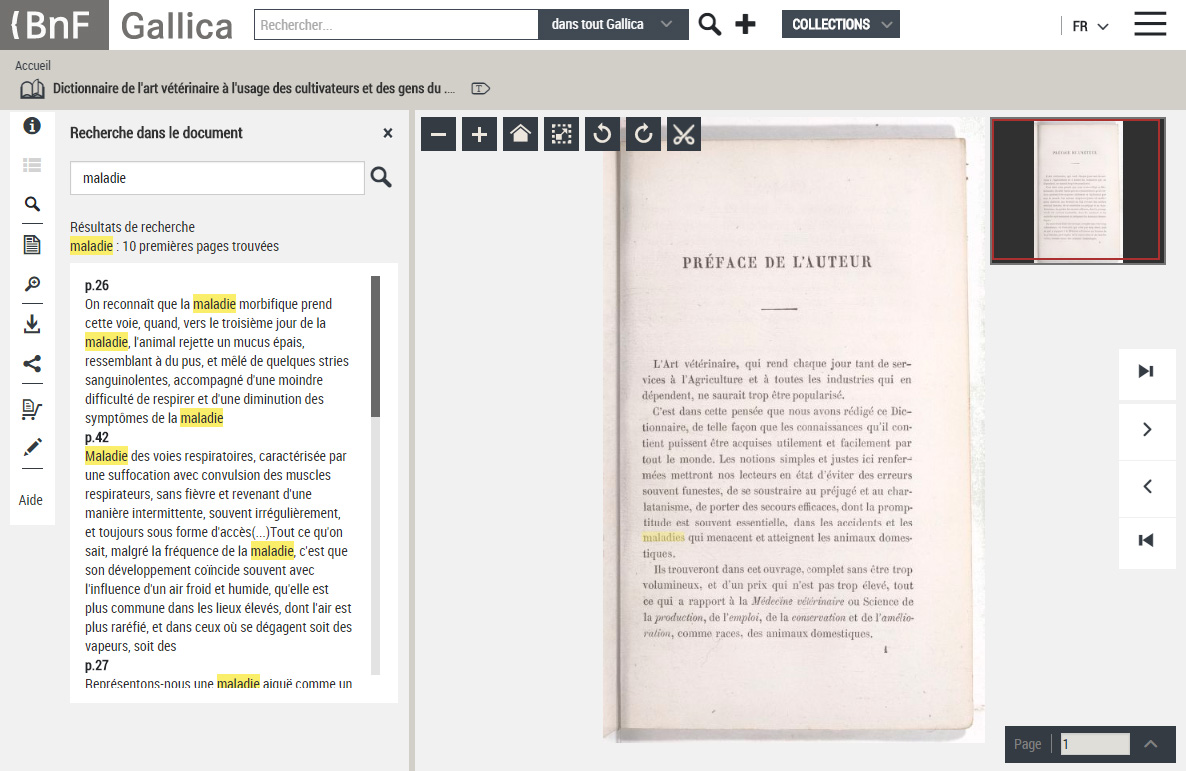
\includegraphics[width=1\textwidth]{figure/screenshot_gallica.jpg}
            \caption{Capture d'écran du moteur de recherche Gallica}
            \label{fig:gallica}
        \end{figure}

        Pour le téléchargement, on peut télécharger le document en entier ou une sélection du document soit en pdf,
        soit en jpeg pour la page en cours. Les options de consultation évoluent aussi en fonction du type de texte.
        Ainsi la légende, recherche dans le document ou table des matières ne sont pas disponible pour tous les ouvrages.
        Pour les manuscrits, par exemple, on n’aura pas accès au texte plein et pour les revues souvent juste la table des matières.
        Outre la visionneuse disponible sur le site web, Gallica propose des applications mobiles sur Google Play et App Store.
        Bien que le site de Gallica soit responsive, l'existence d’application mobile qui imite le site est intéressant.
        Le site ne propose qu’une navigation sommaire entre une série d’image lorsque l’on se rend sur celui-ci depuis un navigateur pour mobile.

        En ce qui concerne la section presse et revues du site plus particulièrement, la visionneuse ne propose
        pas d’options spécifiques à ce type de document. Sur la plupart des revues nous n’avons pas accès à l’OCR
        c’est pourquoi il serait intéressant d’implémenter cette fonctionnalité pour notre projet.

        \subsection{Europeana}
        \label{sec:europeana}
        Europeana est une bibliothèque numérique européenne qui a été lancée en 2008 par la Comission européenne et qui est une mise en commun des ressources,
        ( livres, des images, des vidéos, des photographies… ) des bibliothèques nationales des 27 pays membres. Chose importante à noter,
        le site n’archive pas les œuvres mais sert de catalogue de recherche, fournissant des liens vers l’institution ayant numérisée l’objet 
        (ex : Gallica cité plus haut).

        On peut par ailleurs créer un compte, qui va nous permettre de garder en favoris des « objets », des recherches, des tags,
        des traductions dans d’autres langages… pour pouvoir y revenir plus tard.

        Lors d’une recherche, une auto-complétion propose des recherches similaires ou plus complètes, à la manière de Google
        (ex : écrire ‘napoleon’ va proposer ‘napoleon’ mais aussi ‘napoleon bonaparte’ ‘napoleon I emporor of french’ …).
        Il est possible de rechercher suivant un sujet, un auteur, un titre, une période ou un lieu. Après la recherche,
        les premiers résultats sont proposés et il est possible d’affiner celle-ci, en précisent le type de la recherche
        (image, vidéo, son, texte …), la langue, l'année, le pays, en rajoutant des mots-clés. Mais la recherche permet aussi
        d’obtenir des objets qui sont sous différents copyright… 
        Accéder à un objet fournit des informations sur celui-ci, comme les titres alternatifs, sa description, son type, sa date, les tags générés pour celui-ci,
        la source de l’objet et qui le fournit. On peut ensuite accéder à l’objet par un lien qui retourne sur le site ayant archivé l’élément trouvé.

        Il n’y a pas de réelle interaction avec les documents sur cette plateforme ; le reste se passe sur les diverses plateformes qui ont archivées les éléments.

        Autre élément intéressant, la présence d’Europeana sur Pinterest, mise en avant sur la page d’accueil du site.
        Le site propose en effet de très nombreux tableaux – 98 à l’heure actuelle – avec plus de 3000 épingles qui regroupent
        donc des images, des musiques, des expositions… autour de divers thèmes et qui permet de passer par un autre média que leur plateforme.


        \subsection{archives.morbihan}
        \label{subsec:morbihan}
        Ce site concerne les archives du Morbihan. L’ outils de consultation de presse ancienne est presque semblable
        (en termes de services offerts) à celui proposé par les archives des Yvelines. Le site propose une application
        de filtres sur les documents (comme l’illustre la figure ci-dessous). Il propose aussi une version texte des
        articles de journaux. Cependant il n’est pas possible d’effectuer une recherche sur la version texte,
        alors que c'est assez utile et pratique.

        \subsection{britishnewspaperarchive}
        \label{subsec:britishnewspaper}
        La plate-forme “britishnewspaperarchive” est un site de consultation de presse ancienne du Royaume-Uni.
        Le site comporte près de 12 millions de pages de journaux allant de 1710 à 1959. Il est possible
        d’effectuer une recherche par période, région, pays, ville, ou encore par journal. La consultation
        des journaux est cependant payante à hauteur de £12,95 le mois, ce qui est une véritable contrainte
        pour un utilisateur non régulier.

        \subsection{archive.winnipegfreepress}
        \label{subsec:winnipeg}
        C’est un site américain de consultation de presse ancienne qui permet d’effectuer une recherche par période,
        par thématique, ou par mots-clés. La consultation des journaux ici est aussi payante
        (\$9,18/semaine) . Mais le site propose une période d’essai gratuite de 14 jours donnant accès à tous les documents de presse.

        \subsection{Chronicling America}
        \label{subsec:chrinamerica}
        “Chroniclingamerica” est une plate-forme de consultation de presse ancienne américaine qui offre des services
        tels que le zoom, le rognage, l’impression, le téléchargement sous forme d’image ou pdf. Le site propose
        aussi une consultation du journal sous forme de texte permettant ainsi de faire une recherche classique
        (à l’aide d’un Ctrl+F). Cependant la mise en forme de la version texte du journal ne facilite pas beaucoup la lecture.


    \subsection{Point sur l’état de l’art}
    \label{sec:point}
    L’étude de l’art permet de faire un point sur ce qui existe pour voir ce qu’il serait très intéressant de proposer
    sur la plateforme afin de ne pas proposer moins de fonctionnalités que ce qui existe déjà. Il faut cependant garder
    en tête que nos ressources (temps et développeurs) sont limitées, et que nous ne pourrons peut-être pas tout réaliser ;
    voici cependant les objectifs que l’on a mentionné plus haut qui semblent très important à mettre en place vis-à-vis
    de ce qui existe déjà actuellement.

    \subparagraph{Des interactions sur le document, par nécessité :}
    Fonctionnalités communes à toutes les plateformes et qui sont donc indispensables ;
    il sera nécessaire, sur le document, de pouvoir se déplacer (zoom/dézoom) sur les images trop grandes
    pour l’écran (notamment car les pages de journaux peuvent-être très grandes), télécharger le document.
    Une autre fonctionnalité très intéressante est de pouvoir ‘bookmark’ le document afin de pouvoir
    y revenir directement plus tard à partir de son compte.

    \subparagraph{Recherche plein texte, pour compléter la recherche :}
    Un élément important pour des journaux, dont le contenu par page peut-être énorme - certaines images
    sont plus grandes que 5000x3000 pixels,- et qui n’est pourtant pas présente sur toutes les plateformes :
    permettre de rechercher du texte directement sur la page. L’utilisateur doit pouvoir rechercher du texte,
    et pouvoir retrouver facilement les résultats de sa recherche sur la page qui seront mis en avant directement
    sur la page (résultat entouré / surligné ...).

    \subparagraph{Mise en avant de journaux, pour des propositions ludiques :}
    Archives Yvelines a mis quelque chose d’intéressant en place ; ils proposent en avant des documents
    qui sont sortis 100 an avant jour pour jour. Il serait intéressant de mettre en avant des journaux/articles
    en lien avec des évènements dont l’anniversaire est proche, par exemple.

    \subparagraph{Des parcours thématiques, pour se démarquer des autres :}
    Enfin concernant les fonctionnalités de la plateforme générale, on remarquera que la seule interaction
    présente entre les utilisateurs et les documents sont l’ajout d’annotation pour améliorer la lecture,
    et ce car les OCR utilisés ne sont pas forcément les plus performants. Les utilisateurs peuvent donc apporter
    certaines informations sur certains documents, et c’est tout. Et c’est un point très important à noter,
    qui va permettre de nous démarquer des autres.  La possibilité pour les utilisateurs de créer des parcours thématiques
    devient une tâche primordiale. Ils pourront donc regrouper des articles, des journaux autour de dates, d’évènements...
    ou de tous autres éléments dont il serait intéressant d’avoir plusieurs sources d’information. Enfin il sera très important
    de permettre à divers utilisateurs d’apporter des modifications sur un parcours, de partager ceux-ci, de les mettre en avant.
